\documentclass[1p]{elsarticle_modified}
%\bibliographystyle{elsarticle-num}

%\usepackage[colorlinks]{hyperref}
%\usepackage{abbrmath_seonhwa} %\Abb, \Ascr, \Acal ,\Abf, \Afrak
\usepackage{amsfonts}
\usepackage{amssymb}
\usepackage{amsmath}
\usepackage{amsthm}
\usepackage{scalefnt}
\usepackage{amsbsy}
\usepackage{kotex}
\usepackage{caption}
\usepackage{subfig}
\usepackage{color}
\usepackage{graphicx}
\usepackage{xcolor} %% white, black, red, green, blue, cyan, magenta, yellow
\usepackage{float}
\usepackage{setspace}
\usepackage{hyperref}

\usepackage{tikz}
\usetikzlibrary{arrows}

\usepackage{multirow}
\usepackage{array} % fixed length table
\usepackage{hhline}

%%%%%%%%%%%%%%%%%%%%%
\makeatletter
\renewcommand*\env@matrix[1][\arraystretch]{%
	\edef\arraystretch{#1}%
	\hskip -\arraycolsep
	\let\@ifnextchar\new@ifnextchar
	\array{*\c@MaxMatrixCols c}}
\makeatother %https://tex.stackexchange.com/questions/14071/how-can-i-increase-the-line-spacing-in-a-matrix
%%%%%%%%%%%%%%%

\usepackage[normalem]{ulem}

\newcommand{\msout}[1]{\ifmmode\text{\sout{\ensuremath{#1}}}\else\sout{#1}\fi}
%SOURCE: \msout is \stkout macro in https://tex.stackexchange.com/questions/20609/strikeout-in-math-mode

\newcommand{\cancel}[1]{
	\ifmmode
	{\color{red}\msout{#1}}
	\else
	{\color{red}\sout{#1}}
	\fi
}

\newcommand{\add}[1]{
	{\color{blue}\uwave{#1}}
}

\newcommand{\replace}[2]{
	\ifmmode
	{\color{red}\msout{#1}}{\color{blue}\uwave{#2}}
	\else
	{\color{red}\sout{#1}}{\color{blue}\uwave{#2}}
	\fi
}

\newcommand{\Sol}{\mathcal{S}} %segment
\newcommand{\D}{D} %diagram
\newcommand{\A}{\mathcal{A}} %arc


%%%%%%%%%%%%%%%%%%%%%%%%%%%%%5 test

\def\sl{\operatorname{\textup{SL}}(2,\Cbb)}
\def\psl{\operatorname{\textup{PSL}}(2,\Cbb)}
\def\quan{\mkern 1mu \triangleright \mkern 1mu}

\theoremstyle{definition}
\newtheorem{thm}{Theorem}[section]
\newtheorem{prop}[thm]{Proposition}
\newtheorem{lem}[thm]{Lemma}
\newtheorem{ques}[thm]{Question}
\newtheorem{cor}[thm]{Corollary}
\newtheorem{defn}[thm]{Definition}
\newtheorem{exam}[thm]{Example}
\newtheorem{rmk}[thm]{Remark}
\newtheorem{alg}[thm]{Algorithm}

\newcommand{\I}{\sqrt{-1}}
\begin{document}

%\begin{frontmatter}
%
%\title{Boundary parabolic representations of knots up to 8 crossings}
%
%%% Group authors per affiliation:
%\author{Yunhi Cho} 
%\address{Department of Mathematics, University of Seoul, Seoul, Korea}
%\ead{yhcho@uos.ac.kr}
%
%
%\author{Seonhwa Kim} %\fnref{s_kim}}
%\address{Center for Geometry and Physics, Institute for Basic Science, Pohang, 37673, Korea}
%\ead{ryeona17@ibs.re.kr}
%
%\author{Hyuk Kim}
%\address{Department of Mathematical Sciences, Seoul National University, Seoul 08826, Korea}
%\ead{hyukkim@snu.ac.kr}
%
%\author{Seokbeom Yoon}
%\address{Department of Mathematical Sciences, Seoul National University, Seoul, 08826,  Korea}
%\ead{sbyoon15@snu.ac.kr}
%
%\begin{abstract}
%We find all boundary parabolic representation of knots up to 8 crossings.
%
%\end{abstract}
%\begin{keyword}
%    \MSC[2010] 57M25 
%\end{keyword}
%
%\end{frontmatter}

%\linenumbers
%\tableofcontents
%
\newcommand\colored[1]{\textcolor{white}{\rule[-0.35ex]{0.8em}{1.4ex}}\kern-0.8em\color{red} #1}%
%\newcommand\colored[1]{\textcolor{white}{ #1}\kern-2.17ex	\textcolor{white}{ #1}\kern-1.81ex	\textcolor{white}{ #1}\kern-2.15ex\color{red}#1	}

{\Large $\underline{12a_{0612}~(K12a_{0612})}$}

\setlength{\tabcolsep}{10pt}
\renewcommand{\arraystretch}{1.6}
\vspace{1cm}\begin{tabular}{m{100pt}>{\centering\arraybackslash}m{274pt}}
\multirow{5}{120pt}{
	\centering
	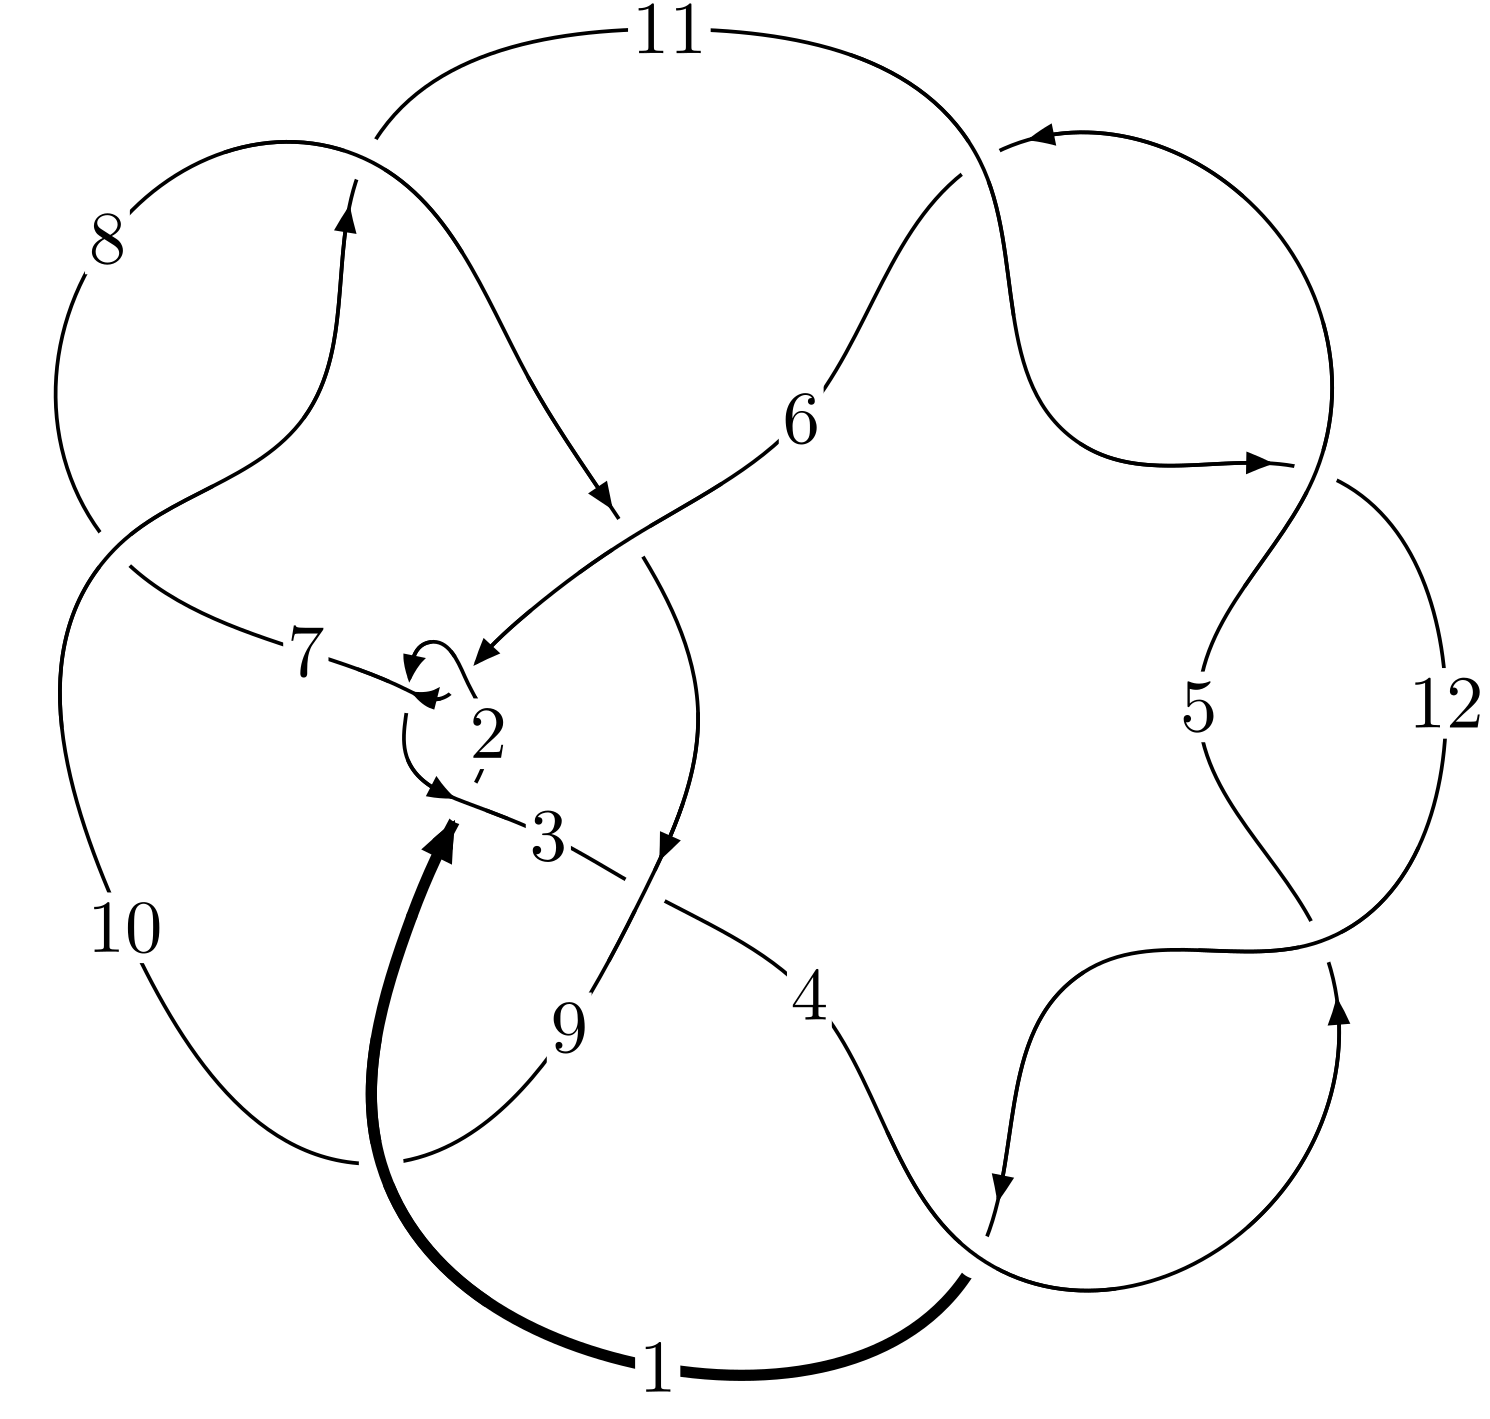
\includegraphics[width=112pt]{../../../GIT/diagram.site/Diagrams/png/1413_12a_0612.png}\\
\ \ \ A knot diagram\footnotemark}&
\allowdisplaybreaks
\textbf{Linearized knot diagam} \\
\cline{2-2}
 &
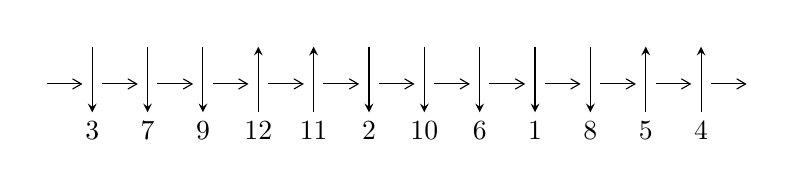
\begin{tikzpicture}[x=20pt, y=17pt]
	% nodes
	\node (C0) at (0, 0) {};
	\node (C1) at (1, 0) {};
	\node (C1U) at (1, +1) {};
	\node (C1D) at (1, -1) {3};

	\node (C2) at (2, 0) {};
	\node (C2U) at (2, +1) {};
	\node (C2D) at (2, -1) {7};

	\node (C3) at (3, 0) {};
	\node (C3U) at (3, +1) {};
	\node (C3D) at (3, -1) {9};

	\node (C4) at (4, 0) {};
	\node (C4U) at (4, +1) {};
	\node (C4D) at (4, -1) {12};

	\node (C5) at (5, 0) {};
	\node (C5U) at (5, +1) {};
	\node (C5D) at (5, -1) {11};

	\node (C6) at (6, 0) {};
	\node (C6U) at (6, +1) {};
	\node (C6D) at (6, -1) {2};

	\node (C7) at (7, 0) {};
	\node (C7U) at (7, +1) {};
	\node (C7D) at (7, -1) {10};

	\node (C8) at (8, 0) {};
	\node (C8U) at (8, +1) {};
	\node (C8D) at (8, -1) {6};

	\node (C9) at (9, 0) {};
	\node (C9U) at (9, +1) {};
	\node (C9D) at (9, -1) {1};

	\node (C10) at (10, 0) {};
	\node (C10U) at (10, +1) {};
	\node (C10D) at (10, -1) {8};

	\node (C11) at (11, 0) {};
	\node (C11U) at (11, +1) {};
	\node (C11D) at (11, -1) {5};

	\node (C12) at (12, 0) {};
	\node (C12U) at (12, +1) {};
	\node (C12D) at (12, -1) {4};
	\node (C13) at (13, 0) {};

	% arrows
	\draw[->,>={angle 60}]
	(C0) edge (C1) (C1) edge (C2) (C2) edge (C3) (C3) edge (C4) (C4) edge (C5) (C5) edge (C6) (C6) edge (C7) (C7) edge (C8) (C8) edge (C9) (C9) edge (C10) (C10) edge (C11) (C11) edge (C12) (C12) edge (C13) ;	\draw[->,>=stealth]
	(C1U) edge (C1D) (C2U) edge (C2D) (C3U) edge (C3D) (C4D) edge (C4U) (C5D) edge (C5U) (C6U) edge (C6D) (C7U) edge (C7D) (C8U) edge (C8D) (C9U) edge (C9D) (C10U) edge (C10D) (C11D) edge (C11U) (C12D) edge (C12U) ;
	\end{tikzpicture} \\
\hhline{~~} \\& 
\textbf{Solving Sequence} \\ \cline{2-2} 
 &
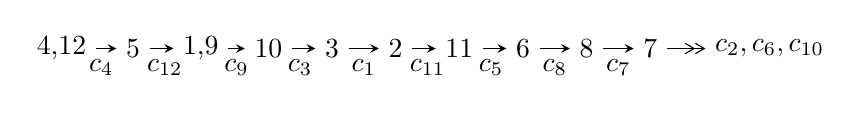
\begin{tikzpicture}[x=23pt, y=7pt]
	% node
	\node (A0) at (-1/8, 0) {4,12};
	\node (A1) at (1, 0) {5};
	\node (A2) at (33/16, 0) {1,9};
	\node (A3) at (25/8, 0) {10};
	\node (A4) at (33/8, 0) {3};
	\node (A5) at (41/8, 0) {2};
	\node (A6) at (49/8, 0) {11};
	\node (A7) at (57/8, 0) {6};
	\node (A8) at (65/8, 0) {8};
	\node (A9) at (73/8, 0) {7};
	\node (C1) at (1/2, -1) {$c_{4}$};
	\node (C2) at (3/2, -1) {$c_{12}$};
	\node (C3) at (21/8, -1) {$c_{9}$};
	\node (C4) at (29/8, -1) {$c_{3}$};
	\node (C5) at (37/8, -1) {$c_{1}$};
	\node (C6) at (45/8, -1) {$c_{11}$};
	\node (C7) at (53/8, -1) {$c_{5}$};
	\node (C8) at (61/8, -1) {$c_{8}$};
	\node (C9) at (69/8, -1) {$c_{7}$};
	\node (A10) at (11, 0) {$c_{2},c_{6},c_{10}$};

	% edge
	\draw[->,>=stealth]	
	(A0) edge (A1) (A1) edge (A2) (A2) edge (A3) (A3) edge (A4) (A4) edge (A5) (A5) edge (A6) (A6) edge (A7) (A7) edge (A8) (A8) edge (A9) ;
	\draw[->>,>={angle 60}]	
	(A9) edge (A10);
\end{tikzpicture} \\ 

\end{tabular} \\

\footnotetext{
The image of knot diagram is generated by the software ``\textbf{Draw programme}" developed by Andrew Bartholomew(\url{http://www.layer8.co.uk/maths/draw/index.htm\#Running-draw}), where we modified some parts for our purpose(\url{https://github.com/CATsTAILs/LinksPainter}).
}\phantom \\ \newline 
\centering \textbf{Ideals for irreducible components\footnotemark of $X_{\text{par}}$} 
 
\begin{align*}
I^u_{1}&=\langle 
-2.18462\times10^{73} u^{73}+3.16063\times10^{73} u^{72}+\cdots+5.40007\times10^{73} b-3.24788\times10^{72},\\
\phantom{I^u_{1}}&\phantom{= \langle  }-2.10222\times10^{73} u^{73}-1.17709\times10^{73} u^{72}+\cdots+2.16003\times10^{74} a-7.97915\times10^{74},\;u^{74}-2 u^{73}+\cdots-5 u+1\rangle \\
I^u_{2}&=\langle 
b,\;2 a+1,\;u^2- u+1\rangle \\
\\
\end{align*}
\raggedright * 2 irreducible components of $\dim_{\mathbb{C}}=0$, with total 76 representations.\\
\footnotetext{All coefficients of polynomials are rational numbers. But the coefficients are sometimes approximated in decimal forms when there is not enough margin.}
\newpage
\renewcommand{\arraystretch}{1}
\centering \section*{I. $I^u_{1}= \langle -2.18\times10^{73} u^{73}+3.16\times10^{73} u^{72}+\cdots+5.40\times10^{73} b-3.25\times10^{72},\;-2.10\times10^{73} u^{73}-1.18\times10^{73} u^{72}+\cdots+2.16\times10^{74} a-7.98\times10^{74},\;u^{74}-2 u^{73}+\cdots-5 u+1 \rangle$}
\flushleft \textbf{(i) Arc colorings}\\
\begin{tabular}{m{7pt} m{180pt} m{7pt} m{180pt} }
\flushright $a_{4}=$&$\begin{pmatrix}1\\0\end{pmatrix}$ \\
\flushright $a_{12}=$&$\begin{pmatrix}0\\u\end{pmatrix}$ \\
\flushright $a_{5}=$&$\begin{pmatrix}1\\- u^2\end{pmatrix}$ \\
\flushright $a_{1}=$&$\begin{pmatrix}u\\u\end{pmatrix}$ \\
\flushright $a_{9}=$&$\begin{pmatrix}0.0973237 u^{73}+0.0544942 u^{72}+\cdots-7.75879 u+3.69400\\0.404554 u^{73}-0.585294 u^{72}+\cdots+2.13148 u+0.0601452\end{pmatrix}$ \\
\flushright $a_{10}=$&$\begin{pmatrix}0.0724192 u^{73}+0.00246463 u^{72}+\cdots-7.32492 u+3.66868\\0.379649 u^{73}-0.637323 u^{72}+\cdots+2.56535 u+0.0348175\end{pmatrix}$ \\
\flushright $a_{3}=$&$\begin{pmatrix}1.52542 u^{73}-2.53855 u^{72}+\cdots+1.82716 u-0.738325\\0.550001 u^{73}-0.984294 u^{72}+\cdots+1.31434 u-0.000117455\end{pmatrix}$ \\
\flushright $a_{2}=$&$\begin{pmatrix}-1.45206 u^{73}+3.42469 u^{72}+\cdots-9.87487 u+1.52722\\-0.301071 u^{73}+0.447914 u^{72}+\cdots+0.617849 u-0.0822885\end{pmatrix}$ \\
\flushright $a_{11}=$&$\begin{pmatrix}- u\\u^3+u\end{pmatrix}$ \\
\flushright $a_{6}=$&$\begin{pmatrix}u^2+1\\- u^4-2 u^2\end{pmatrix}$ \\
\flushright $a_{8}=$&$\begin{pmatrix}-0.317026 u^{73}+0.923011 u^{72}+\cdots-6.65577 u+3.92960\\0.433026 u^{73}-1.09679 u^{72}+\cdots+4.34853 u-0.519695\end{pmatrix}$ \\
\flushright $a_{7}=$&$\begin{pmatrix}-0.512410 u^{73}+1.28277 u^{72}+\cdots+1.89759 u+0.211662\\0.0303919 u^{73}-0.875961 u^{72}+\cdots+5.08662 u-1.26747\end{pmatrix}$\\&\end{tabular}
\flushleft \textbf{(ii) Obstruction class $= -1$}\\~\\
\flushleft \textbf{(iii) Cusp Shapes $= 6.42891 u^{73}-17.1405 u^{72}+\cdots+84.2991 u-27.4117$}\\~\\
\newpage\renewcommand{\arraystretch}{1}
\flushleft \textbf{(iv) u-Polynomials at the component}\newline \\
\begin{tabular}{m{50pt}|m{274pt}}
Crossings & \hspace{64pt}u-Polynomials at each crossing \\
\hline $$\begin{aligned}c_{1}\end{aligned}$$&$\begin{aligned}
&u^{74}+30 u^{73}+\cdots+11 u+1
\end{aligned}$\\
\hline $$\begin{aligned}c_{2},c_{6}\end{aligned}$$&$\begin{aligned}
&u^{74}-2 u^{73}+\cdots+u+1
\end{aligned}$\\
\hline $$\begin{aligned}c_{3}\end{aligned}$$&$\begin{aligned}
&u^{74}- u^{73}+\cdots+32 u-64
\end{aligned}$\\
\hline $$\begin{aligned}c_{4},c_{5},c_{11}\\c_{12}\end{aligned}$$&$\begin{aligned}
&u^{74}+2 u^{73}+\cdots+5 u+1
\end{aligned}$\\
\hline $$\begin{aligned}c_{7},c_{10}\end{aligned}$$&$\begin{aligned}
&u^{74}-3 u^{73}+\cdots-24 u-16
\end{aligned}$\\
\hline $$\begin{aligned}c_{8}\end{aligned}$$&$\begin{aligned}
&4(4 u^{74}+50 u^{73}+\cdots+1.01760\times10^{7} u-826861)
\end{aligned}$\\
\hline $$\begin{aligned}c_{9}\end{aligned}$$&$\begin{aligned}
&4(4 u^{74}+74 u^{73}+\cdots+3578 u+331)
\end{aligned}$\\
\hline
\end{tabular}\\~\\
\newpage\renewcommand{\arraystretch}{1}
\flushleft \textbf{(v) Riley Polynomials at the component}\newline \\
\begin{tabular}{m{50pt}|m{274pt}}
Crossings & \hspace{64pt}Riley Polynomials at each crossing \\
\hline $$\begin{aligned}c_{1}\end{aligned}$$&$\begin{aligned}
&y^{74}+22 y^{73}+\cdots-11 y+1
\end{aligned}$\\
\hline $$\begin{aligned}c_{2},c_{6}\end{aligned}$$&$\begin{aligned}
&y^{74}-30 y^{73}+\cdots-11 y+1
\end{aligned}$\\
\hline $$\begin{aligned}c_{3}\end{aligned}$$&$\begin{aligned}
&y^{74}-15 y^{73}+\cdots-100864 y+4096
\end{aligned}$\\
\hline $$\begin{aligned}c_{4},c_{5},c_{11}\\c_{12}\end{aligned}$$&$\begin{aligned}
&y^{74}+90 y^{73}+\cdots-11 y+1
\end{aligned}$\\
\hline $$\begin{aligned}c_{7},c_{10}\end{aligned}$$&$\begin{aligned}
&y^{74}-57 y^{73}+\cdots+8928 y+256
\end{aligned}$\\
\hline $$\begin{aligned}c_{8}\end{aligned}$$&$\begin{aligned}
&16(16 y^{74}-988 y^{73}+\cdots-3.20264\times10^{13} y+6.83699\times10^{11})
\end{aligned}$\\
\hline $$\begin{aligned}c_{9}\end{aligned}$$&$\begin{aligned}
&16(16 y^{74}-12 y^{73}+\cdots-4095460 y+109561)
\end{aligned}$\\
\hline
\end{tabular}\\~\\
\newpage\flushleft \textbf{(vi) Complex Volumes and Cusp Shapes}
$$\begin{array}{c|c|c}  
\text{Solutions to }I^u_{1}& \I (\text{vol} + \sqrt{-1}CS) & \text{Cusp shape}\\
 \hline 
\begin{aligned}
u &= \phantom{-}0.516398 + 0.937796 I \\
a &= \phantom{-}1.37934 + 0.47440 I \\
b &= \phantom{-}1.11519 - 1.02621 I\end{aligned}
 & -5.3318 + 13.4301 I & \phantom{-0.000000 } 0 \\ \hline\begin{aligned}
u &= \phantom{-}0.516398 - 0.937796 I \\
a &= \phantom{-}1.37934 - 0.47440 I \\
b &= \phantom{-}1.11519 + 1.02621 I\end{aligned}
 & -5.3318 - 13.4301 I & \phantom{-0.000000 } 0 \\ \hline\begin{aligned}
u &= \phantom{-}0.646355 + 0.860532 I \\
a &= -0.031559 + 0.651495 I \\
b &= \phantom{-}0.787715 + 0.427271 I\end{aligned}
 & -4.52765 - 4.39825 I & \phantom{-0.000000 } 0 \\ \hline\begin{aligned}
u &= \phantom{-}0.646355 - 0.860532 I \\
a &= -0.031559 - 0.651495 I \\
b &= \phantom{-}0.787715 - 0.427271 I\end{aligned}
 & -4.52765 + 4.39825 I & \phantom{-0.000000 } 0 \\ \hline\begin{aligned}
u &= -0.514593 + 0.957275 I \\
a &= -1.203500 + 0.319270 I \\
b &= -0.931893 - 0.901069 I\end{aligned}
 & -3.14453 - 7.64245 I & \phantom{-0.000000 } 0 \\ \hline\begin{aligned}
u &= -0.514593 - 0.957275 I \\
a &= -1.203500 - 0.319270 I \\
b &= -0.931893 + 0.901069 I\end{aligned}
 & -3.14453 + 7.64245 I & \phantom{-0.000000 } 0 \\ \hline\begin{aligned}
u &= -0.164439 + 1.088400 I \\
a &= -0.289406 - 0.798790 I \\
b &= \phantom{-}0.007352 - 0.649980 I\end{aligned}
 & -0.76278 - 2.78369 I & \phantom{-0.000000 } 0 \\ \hline\begin{aligned}
u &= -0.164439 - 1.088400 I \\
a &= -0.289406 + 0.798790 I \\
b &= \phantom{-}0.007352 + 0.649980 I\end{aligned}
 & -0.76278 + 2.78369 I & \phantom{-0.000000 } 0 \\ \hline\begin{aligned}
u &= \phantom{-}0.565708 + 0.953078 I \\
a &= \phantom{-}0.797027 + 0.611956 I \\
b &= \phantom{-}1.083310 - 0.435515 I\end{aligned}
 & -9.49521 + 4.75713 I & \phantom{-0.000000 } 0 \\ \hline\begin{aligned}
u &= \phantom{-}0.565708 - 0.953078 I \\
a &= \phantom{-}0.797027 - 0.611956 I \\
b &= \phantom{-}1.083310 + 0.435515 I\end{aligned}
 & -9.49521 - 4.75713 I & \phantom{-0.000000 } 0\\
 \hline 
 \end{array}$$\newpage$$\begin{array}{c|c|c}  
\text{Solutions to }I^u_{1}& \I (\text{vol} + \sqrt{-1}CS) & \text{Cusp shape}\\
 \hline 
\begin{aligned}
u &= -0.139200 + 0.868293 I \\
a &= \phantom{-}1.067450 - 0.566161 I \\
b &= \phantom{-}1.41905 - 1.07046 I\end{aligned}
 & -5.34190 - 5.03781 I & \phantom{-0.000000 } 0 \\ \hline\begin{aligned}
u &= -0.139200 - 0.868293 I \\
a &= \phantom{-}1.067450 + 0.566161 I \\
b &= \phantom{-}1.41905 + 1.07046 I\end{aligned}
 & -5.34190 + 5.03781 I & \phantom{-0.000000 } 0 \\ \hline\begin{aligned}
u &= -0.053293 + 0.873796 I \\
a &= \phantom{-}0.463556 - 0.288559 I \\
b &= \phantom{-}0.57959 - 1.54839 I\end{aligned}
 & -6.12072 + 1.15020 I & \phantom{-0.000000 } 0 \\ \hline\begin{aligned}
u &= -0.053293 - 0.873796 I \\
a &= \phantom{-}0.463556 + 0.288559 I \\
b &= \phantom{-}0.57959 + 1.54839 I\end{aligned}
 & -6.12072 - 1.15020 I & \phantom{-0.000000 } 0 \\ \hline\begin{aligned}
u &= \phantom{-}0.339838 + 0.799583 I \\
a &= -1.61362 - 0.26065 I \\
b &= -1.24870 + 1.11169 I\end{aligned}
 & -0.75369 + 7.61744 I & \phantom{-0.000000 } 0 \\ \hline\begin{aligned}
u &= \phantom{-}0.339838 - 0.799583 I \\
a &= -1.61362 + 0.26065 I \\
b &= -1.24870 - 1.11169 I\end{aligned}
 & -0.75369 - 7.61744 I & \phantom{-0.000000 } 0 \\ \hline\begin{aligned}
u &= \phantom{-}0.857154\phantom{ +0.000000I} \\
a &= \phantom{-}0.267986\phantom{ +0.000000I} \\
b &= -0.915149\phantom{ +0.000000I}\end{aligned}
 & -6.54255\phantom{ +0.000000I} & -13.9400\phantom{ +0.000000I} \\ \hline\begin{aligned}
u &= -0.352195 + 0.760005 I \\
a &= \phantom{-}1.41551 - 0.20271 I \\
b &= \phantom{-}0.886656 + 1.011220 I\end{aligned}
 & \phantom{-}0.71510 - 2.68070 I & \phantom{-0.000000 } 0 \\ \hline\begin{aligned}
u &= -0.352195 - 0.760005 I \\
a &= \phantom{-}1.41551 + 0.20271 I \\
b &= \phantom{-}0.886656 - 1.011220 I\end{aligned}
 & \phantom{-}0.71510 + 2.68070 I & \phantom{-0.000000 } 0 \\ \hline\begin{aligned}
u &= -0.809015 + 0.119912 I \\
a &= -0.063657 - 0.319788 I \\
b &= \phantom{-}0.625904 + 0.637596 I\end{aligned}
 & \phantom{-}0.12891 - 3.27306 I & \phantom{-0.000000 -}0. + 6.36577 I\\
 \hline 
 \end{array}$$\newpage$$\begin{array}{c|c|c}  
\text{Solutions to }I^u_{1}& \I (\text{vol} + \sqrt{-1}CS) & \text{Cusp shape}\\
 \hline 
\begin{aligned}
u &= -0.809015 - 0.119912 I \\
a &= -0.063657 + 0.319788 I \\
b &= \phantom{-}0.625904 - 0.637596 I\end{aligned}
 & \phantom{-}0.12891 + 3.27306 I & \phantom{-0.000000 } 0. - 6.36577 I \\ \hline\begin{aligned}
u &= \phantom{-}0.229003 + 0.780373 I \\
a &= -1.50737 - 0.57430 I \\
b &= -1.213480 + 0.110904 I\end{aligned}
 & -3.53186 + 1.82003 I & -12.85757 + 0. I\phantom{ +0.000000I} \\ \hline\begin{aligned}
u &= \phantom{-}0.229003 - 0.780373 I \\
a &= -1.50737 + 0.57430 I \\
b &= -1.213480 - 0.110904 I\end{aligned}
 & -3.53186 - 1.82003 I & -12.85757 + 0. I\phantom{ +0.000000I} \\ \hline\begin{aligned}
u &= \phantom{-}0.116450 + 0.799438 I \\
a &= -1.337450 - 0.093652 I \\
b &= -0.844614 - 0.673886 I\end{aligned}
 & -3.46518 + 1.28856 I & -10.13108 + 0. I\phantom{ +0.000000I} \\ \hline\begin{aligned}
u &= \phantom{-}0.116450 - 0.799438 I \\
a &= -1.337450 + 0.093652 I \\
b &= -0.844614 + 0.673886 I\end{aligned}
 & -3.46518 - 1.28856 I & -10.13108 + 0. I\phantom{ +0.000000I} \\ \hline\begin{aligned}
u &= -0.732025 + 0.956216 I \\
a &= -0.160761 + 0.324928 I \\
b &= -0.525729 + 0.071221 I\end{aligned}
 & -2.08683 - 1.93469 I & \phantom{-0.000000 } 0 \\ \hline\begin{aligned}
u &= -0.732025 - 0.956216 I \\
a &= -0.160761 - 0.324928 I \\
b &= -0.525729 - 0.071221 I\end{aligned}
 & -2.08683 + 1.93469 I & \phantom{-0.000000 } 0 \\ \hline\begin{aligned}
u &= \phantom{-}0.782596 + 0.075119 I \\
a &= \phantom{-}0.210771 - 0.453706 I \\
b &= -0.903700 + 0.805460 I\end{aligned}
 & -2.24768 + 9.11251 I & -6.74714 - 7.64665 I \\ \hline\begin{aligned}
u &= \phantom{-}0.782596 - 0.075119 I \\
a &= \phantom{-}0.210771 + 0.453706 I \\
b &= -0.903700 - 0.805460 I\end{aligned}
 & -2.24768 - 9.11251 I & -6.74714 + 7.64665 I \\ \hline\begin{aligned}
u &= \phantom{-}0.157717 + 0.755447 I \\
a &= -0.07570 - 1.57177 I \\
b &= -0.364346 - 0.324652 I\end{aligned}
 & -1.00910 - 2.34681 I & -6.98279 + 1.27218 I\\
 \hline 
 \end{array}$$\newpage$$\begin{array}{c|c|c}  
\text{Solutions to }I^u_{1}& \I (\text{vol} + \sqrt{-1}CS) & \text{Cusp shape}\\
 \hline 
\begin{aligned}
u &= \phantom{-}0.157717 - 0.755447 I \\
a &= -0.07570 + 1.57177 I \\
b &= -0.364346 + 0.324652 I\end{aligned}
 & -1.00910 + 2.34681 I & -6.98279 - 1.27218 I \\ \hline\begin{aligned}
u &= -0.315752 + 0.567010 I \\
a &= \phantom{-}0.726247 - 0.417162 I \\
b &= \phantom{-}0.265687 + 0.485420 I\end{aligned}
 & -0.095251 - 1.249930 I & -1.34438 + 5.11849 I \\ \hline\begin{aligned}
u &= -0.315752 - 0.567010 I \\
a &= \phantom{-}0.726247 + 0.417162 I \\
b &= \phantom{-}0.265687 - 0.485420 I\end{aligned}
 & -0.095251 + 1.249930 I & -1.34438 - 5.11849 I \\ \hline\begin{aligned}
u &= \phantom{-}0.120112 + 0.600674 I \\
a &= -4.25050 - 3.90612 I \\
b &= -0.378236 + 0.135229 I\end{aligned}
 & -2.57143 + 1.88701 I & -22.8777 - 20.8815 I \\ \hline\begin{aligned}
u &= \phantom{-}0.120112 - 0.600674 I \\
a &= -4.25050 + 3.90612 I \\
b &= -0.378236 - 0.135229 I\end{aligned}
 & -2.57143 - 1.88701 I & -22.8777 + 20.8815 I \\ \hline\begin{aligned}
u &= -0.525480 + 0.097303 I \\
a &= \phantom{-}0.694323 - 0.276907 I \\
b &= -0.448154 + 0.890040 I\end{aligned}
 & \phantom{-}2.69534 - 0.34676 I & \phantom{-}2.07291 + 1.95664 I \\ \hline\begin{aligned}
u &= -0.525480 - 0.097303 I \\
a &= \phantom{-}0.694323 + 0.276907 I \\
b &= -0.448154 - 0.890040 I\end{aligned}
 & \phantom{-}2.69534 + 0.34676 I & \phantom{-}2.07291 - 1.95664 I \\ \hline\begin{aligned}
u &= \phantom{-}0.508981 + 0.034990 I \\
a &= -0.944097 - 0.159201 I \\
b &= \phantom{-}0.768623 + 0.882121 I\end{aligned}
 & \phantom{-}1.52983 - 4.69247 I & -0.63478 + 4.64507 I \\ \hline\begin{aligned}
u &= \phantom{-}0.508981 - 0.034990 I \\
a &= -0.944097 + 0.159201 I \\
b &= \phantom{-}0.768623 - 0.882121 I\end{aligned}
 & \phantom{-}1.52983 + 4.69247 I & -0.63478 - 4.64507 I \\ \hline\begin{aligned}
u &= -0.06618 + 1.61043 I \\
a &= -1.103590 - 0.029524 I \\
b &= -0.610671 - 0.632639 I\end{aligned}
 & -7.73703 - 2.51040 I & \phantom{-0.000000 } 0\\
 \hline 
 \end{array}$$\newpage$$\begin{array}{c|c|c}  
\text{Solutions to }I^u_{1}& \I (\text{vol} + \sqrt{-1}CS) & \text{Cusp shape}\\
 \hline 
\begin{aligned}
u &= -0.06618 - 1.61043 I \\
a &= -1.103590 + 0.029524 I \\
b &= -0.610671 + 0.632639 I\end{aligned}
 & -7.73703 + 2.51040 I & \phantom{-0.000000 } 0 \\ \hline\begin{aligned}
u &= \phantom{-}0.03509 + 1.61351 I \\
a &= \phantom{-}0.888518 + 0.804947 I \\
b &= \phantom{-}0.456223 - 0.165796 I\end{aligned}
 & -9.06255 - 1.74034 I & \phantom{-0.000000 } 0 \\ \hline\begin{aligned}
u &= \phantom{-}0.03509 - 1.61351 I \\
a &= \phantom{-}0.888518 - 0.804947 I \\
b &= \phantom{-}0.456223 + 0.165796 I\end{aligned}
 & -9.06255 + 1.74034 I & \phantom{-0.000000 } 0 \\ \hline\begin{aligned}
u &= \phantom{-}0.00915 + 1.62932 I \\
a &= \phantom{-}3.65614 - 2.49513 I \\
b &= \phantom{-}0.235207 + 0.261485 I\end{aligned}
 & -10.53390 + 2.15468 I & \phantom{-0.000000 } 0 \\ \hline\begin{aligned}
u &= \phantom{-}0.00915 - 1.62932 I \\
a &= \phantom{-}3.65614 + 2.49513 I \\
b &= \phantom{-}0.235207 - 0.261485 I\end{aligned}
 & -10.53390 - 2.15468 I & \phantom{-0.000000 } 0 \\ \hline\begin{aligned}
u &= -0.162962 + 0.325759 I \\
a &= \phantom{-}0.37499 - 5.29235 I \\
b &= -0.061683 + 0.638217 I\end{aligned}
 & -2.74823 + 1.72250 I & \phantom{-}2.01945 - 1.32528 I \\ \hline\begin{aligned}
u &= -0.162962 - 0.325759 I \\
a &= \phantom{-}0.37499 + 5.29235 I \\
b &= -0.061683 - 0.638217 I\end{aligned}
 & -2.74823 - 1.72250 I & \phantom{-}2.01945 + 1.32528 I \\ \hline\begin{aligned}
u &= -0.307838 + 0.186179 I \\
a &= \phantom{-}0.36310 - 3.03306 I \\
b &= -0.728206 + 0.583603 I\end{aligned}
 & -2.23234 - 3.57955 I & -4.32988 + 5.24615 I \\ \hline\begin{aligned}
u &= -0.307838 - 0.186179 I \\
a &= \phantom{-}0.36310 + 3.03306 I \\
b &= -0.728206 - 0.583603 I\end{aligned}
 & -2.23234 + 3.57955 I & -4.32988 - 5.24615 I \\ \hline\begin{aligned}
u &= -0.08246 + 1.64390 I \\
a &= -1.79296 - 0.55515 I \\
b &= -1.26542 - 1.17285 I\end{aligned}
 & -7.63678 - 4.24546 I & \phantom{-0.000000 } 0\\
 \hline 
 \end{array}$$\newpage$$\begin{array}{c|c|c}  
\text{Solutions to }I^u_{1}& \I (\text{vol} + \sqrt{-1}CS) & \text{Cusp shape}\\
 \hline 
\begin{aligned}
u &= -0.08246 - 1.64390 I \\
a &= -1.79296 + 0.55515 I \\
b &= -1.26542 + 1.17285 I\end{aligned}
 & -7.63678 + 4.24546 I & \phantom{-0.000000 } 0 \\ \hline\begin{aligned}
u &= \phantom{-}0.05737 + 1.65209 I \\
a &= \phantom{-}2.06972 + 0.11611 I \\
b &= \phantom{-}1.64431 - 0.28908 I\end{aligned}
 & -12.05210 + 2.87915 I & \phantom{-0.000000 } 0 \\ \hline\begin{aligned}
u &= \phantom{-}0.05737 - 1.65209 I \\
a &= \phantom{-}2.06972 - 0.11611 I \\
b &= \phantom{-}1.64431 + 0.28908 I\end{aligned}
 & -12.05210 - 2.87915 I & \phantom{-0.000000 } 0 \\ \hline\begin{aligned}
u &= \phantom{-}0.08286 + 1.65467 I \\
a &= \phantom{-}2.11845 - 0.66031 I \\
b &= \phantom{-}1.64239 - 1.35516 I\end{aligned}
 & -9.30194 + 9.17519 I & \phantom{-0.000000 } 0 \\ \hline\begin{aligned}
u &= \phantom{-}0.08286 - 1.65467 I \\
a &= \phantom{-}2.11845 + 0.66031 I \\
b &= \phantom{-}1.64239 + 1.35516 I\end{aligned}
 & -9.30194 - 9.17519 I & \phantom{-0.000000 } 0 \\ \hline\begin{aligned}
u &= \phantom{-}0.02506 + 1.66126 I \\
a &= \phantom{-}1.51899 + 0.63274 I \\
b &= \phantom{-}1.15850 + 1.07316 I\end{aligned}
 & -12.15050 + 1.78914 I & \phantom{-0.000000 } 0 \\ \hline\begin{aligned}
u &= \phantom{-}0.02506 - 1.66126 I \\
a &= \phantom{-}1.51899 - 0.63274 I \\
b &= \phantom{-}1.15850 - 1.07316 I\end{aligned}
 & -12.15050 - 1.78914 I & \phantom{-0.000000 } 0 \\ \hline\begin{aligned}
u &= \phantom{-}0.331439 + 0.062097 I \\
a &= \phantom{-}0.042259 - 1.155080 I \\
b &= \phantom{-}0.772329 + 0.069502 I\end{aligned}
 & -1.180990 - 0.117604 I & -4.18793 - 0.25289 I \\ \hline\begin{aligned}
u &= \phantom{-}0.331439 - 0.062097 I \\
a &= \phantom{-}0.042259 + 1.155080 I \\
b &= \phantom{-}0.772329 - 0.069502 I\end{aligned}
 & -1.180990 + 0.117604 I & -4.18793 + 0.25289 I \\ \hline\begin{aligned}
u &= -0.03137 + 1.67412 I \\
a &= -1.88894 + 1.15601 I \\
b &= -1.88611 + 1.43903 I\end{aligned}
 & -14.3020 - 5.6642 I & \phantom{-0.000000 } 0\\
 \hline 
 \end{array}$$\newpage$$\begin{array}{c|c|c}  
\text{Solutions to }I^u_{1}& \I (\text{vol} + \sqrt{-1}CS) & \text{Cusp shape}\\
 \hline 
\begin{aligned}
u &= -0.03137 - 1.67412 I \\
a &= -1.88894 - 1.15601 I \\
b &= -1.88611 - 1.43903 I\end{aligned}
 & -14.3020 + 5.6642 I & \phantom{-0.000000 } 0 \\ \hline\begin{aligned}
u &= -0.01286 + 1.67510 I \\
a &= -0.86416 + 1.39905 I \\
b &= -0.84742 + 2.08208 I\end{aligned}
 & -15.1137 + 0.9015 I & \phantom{-0.000000 } 0 \\ \hline\begin{aligned}
u &= -0.01286 - 1.67510 I \\
a &= -0.86416 - 1.39905 I \\
b &= -0.84742 - 2.08208 I\end{aligned}
 & -15.1137 - 0.9015 I & \phantom{-0.000000 } 0 \\ \hline\begin{aligned}
u &= \phantom{-}0.14686 + 1.69181 I \\
a &= -1.85665 + 0.23574 I \\
b &= -1.30389 + 1.18234 I\end{aligned}
 & -14.4226 + 16.0595 I & \phantom{-0.000000 } 0 \\ \hline\begin{aligned}
u &= \phantom{-}0.14686 - 1.69181 I \\
a &= -1.85665 - 0.23574 I \\
b &= -1.30389 - 1.18234 I\end{aligned}
 & -14.4226 - 16.0595 I & \phantom{-0.000000 } 0 \\ \hline\begin{aligned}
u &= -0.14591 + 1.69645 I \\
a &= \phantom{-}1.68010 + 0.24966 I \\
b &= \phantom{-}1.17315 + 1.05919 I\end{aligned}
 & -12.3248 - 10.2734 I & \phantom{-0.000000 } 0 \\ \hline\begin{aligned}
u &= -0.14591 - 1.69645 I \\
a &= \phantom{-}1.68010 - 0.24966 I \\
b &= \phantom{-}1.17315 - 1.05919 I\end{aligned}
 & -12.3248 + 10.2734 I & \phantom{-0.000000 } 0 \\ \hline\begin{aligned}
u &= \phantom{-}0.15685 + 1.69894 I \\
a &= -1.54459 - 0.10686 I \\
b &= -1.33263 + 0.70962 I\end{aligned}
 & -18.6532 + 7.6097 I & \phantom{-0.000000 } 0 \\ \hline\begin{aligned}
u &= \phantom{-}0.15685 - 1.69894 I \\
a &= -1.54459 + 0.10686 I \\
b &= -1.33263 - 0.70962 I\end{aligned}
 & -18.6532 - 7.6097 I & \phantom{-0.000000 } 0 \\ \hline\begin{aligned}
u &= \phantom{-}0.19047 + 1.71554 I \\
a &= -0.819798 - 0.305915 I \\
b &= -0.900938 + 0.096382 I\end{aligned}
 & -13.42310 - 0.97072 I & \phantom{-0.000000 } 0\\
 \hline 
 \end{array}$$\newpage$$\begin{array}{c|c|c}  
\text{Solutions to }I^u_{1}& \I (\text{vol} + \sqrt{-1}CS) & \text{Cusp shape}\\
 \hline 
\begin{aligned}
u &= \phantom{-}0.19047 - 1.71554 I \\
a &= -0.819798 + 0.305915 I \\
b &= -0.900938 - 0.096382 I\end{aligned}
 & -13.42310 + 0.97072 I & \phantom{-0.000000 } 0 \\ \hline\begin{aligned}
u &= -0.16188 + 1.72459 I \\
a &= \phantom{-}1.005060 + 0.026326 I \\
b &= \phantom{-}0.852608 + 0.458742 I\end{aligned}
 & -11.56300 - 5.35029 I & \phantom{-0.000000 } 0 \\ \hline\begin{aligned}
u &= -0.16188 - 1.72459 I \\
a &= \phantom{-}1.005060 - 0.026326 I \\
b &= \phantom{-}0.852608 - 0.458742 I\end{aligned}
 & -11.56300 + 5.35029 I & \phantom{-0.000000 } 0 \\ \hline\begin{aligned}
u &= \phantom{-}0.261116\phantom{ +0.000000I} \\
a &= \phantom{-}1.48550\phantom{ +0.000000I} \\
b &= \phantom{-}0.559178\phantom{ +0.000000I}\end{aligned}
 & -1.16884\phantom{ +0.000000I} & -7.32880\phantom{ +0.000000I}\\
 \hline 
 \end{array}$$\newpage\newpage\renewcommand{\arraystretch}{1}
\centering \section*{II. $I^u_{2}= \langle b,\;2 a+1,\;u^2- u+1 \rangle$}
\flushleft \textbf{(i) Arc colorings}\\
\begin{tabular}{m{7pt} m{180pt} m{7pt} m{180pt} }
\flushright $a_{4}=$&$\begin{pmatrix}1\\0\end{pmatrix}$ \\
\flushright $a_{12}=$&$\begin{pmatrix}0\\u\end{pmatrix}$ \\
\flushright $a_{5}=$&$\begin{pmatrix}1\\- u+1\end{pmatrix}$ \\
\flushright $a_{1}=$&$\begin{pmatrix}u\\u\end{pmatrix}$ \\
\flushright $a_{9}=$&$\begin{pmatrix}-0.5\\0\end{pmatrix}$ \\
\flushright $a_{10}=$&$\begin{pmatrix}-\frac{1}{2} u\\-\frac{1}{2} u+\frac{1}{2}\end{pmatrix}$ \\
\flushright $a_{3}=$&$\begin{pmatrix}1\\0\end{pmatrix}$ \\
\flushright $a_{2}=$&$\begin{pmatrix}0\\u\end{pmatrix}$ \\
\flushright $a_{11}=$&$\begin{pmatrix}- u\\u-1\end{pmatrix}$ \\
\flushright $a_{6}=$&$\begin{pmatrix}u\\- u+2\end{pmatrix}$ \\
\flushright $a_{8}=$&$\begin{pmatrix}\frac{1}{2} u\\-\frac{3}{2} u+\frac{3}{2}\end{pmatrix}$ \\
\flushright $a_{7}=$&$\begin{pmatrix}u\\- u+1\end{pmatrix}$\\&\end{tabular}
\flushleft \textbf{(ii) Obstruction class $= 1$}\\~\\
\flushleft \textbf{(iii) Cusp Shapes $= -4 u-\frac{7}{4}$}\\~\\
\newpage\renewcommand{\arraystretch}{1}
\flushleft \textbf{(iv) u-Polynomials at the component}\newline \\
\begin{tabular}{m{50pt}|m{274pt}}
Crossings & \hspace{64pt}u-Polynomials at each crossing \\
\hline $$\begin{aligned}c_{1},c_{6},c_{11}\\c_{12}\end{aligned}$$&$\begin{aligned}
&u^2+u+1
\end{aligned}$\\
\hline $$\begin{aligned}c_{2},c_{4},c_{5}\end{aligned}$$&$\begin{aligned}
&u^2- u+1
\end{aligned}$\\
\hline $$\begin{aligned}c_{3}\end{aligned}$$&$\begin{aligned}
&u^2
\end{aligned}$\\
\hline $$\begin{aligned}c_{7}\end{aligned}$$&$\begin{aligned}
&(u-1)^2
\end{aligned}$\\
\hline $$\begin{aligned}c_{8}\end{aligned}$$&$\begin{aligned}
&4(4 u^2+6 u+3)
\end{aligned}$\\
\hline $$\begin{aligned}c_{9}\end{aligned}$$&$\begin{aligned}
&4(4 u^2+2 u+1)
\end{aligned}$\\
\hline $$\begin{aligned}c_{10}\end{aligned}$$&$\begin{aligned}
&(u+1)^2
\end{aligned}$\\
\hline
\end{tabular}\\~\\
\newpage\renewcommand{\arraystretch}{1}
\flushleft \textbf{(v) Riley Polynomials at the component}\newline \\
\begin{tabular}{m{50pt}|m{274pt}}
Crossings & \hspace{64pt}Riley Polynomials at each crossing \\
\hline $$\begin{aligned}c_{1},c_{2},c_{4}\\c_{5},c_{6},c_{11}\\c_{12}\end{aligned}$$&$\begin{aligned}
&y^2+y+1
\end{aligned}$\\
\hline $$\begin{aligned}c_{3}\end{aligned}$$&$\begin{aligned}
&y^2
\end{aligned}$\\
\hline $$\begin{aligned}c_{7},c_{10}\end{aligned}$$&$\begin{aligned}
&(y-1)^2
\end{aligned}$\\
\hline $$\begin{aligned}c_{8}\end{aligned}$$&$\begin{aligned}
&16(16 y^2-12 y+9)
\end{aligned}$\\
\hline $$\begin{aligned}c_{9}\end{aligned}$$&$\begin{aligned}
&16(16 y^2+4 y+1)
\end{aligned}$\\
\hline
\end{tabular}\\~\\
\newpage\flushleft \textbf{(vi) Complex Volumes and Cusp Shapes}
$$\begin{array}{c|c|c}  
\text{Solutions to }I^u_{2}& \I (\text{vol} + \sqrt{-1}CS) & \text{Cusp shape}\\
 \hline 
\begin{aligned}
u &= \phantom{-}0.500000 + 0.866025 I \\
a &= -0.500000\phantom{ +0.000000I} \\
b &= \phantom{-0.000000 } 0\end{aligned}
 & -1.64493 + 2.02988 I & -3.75000 - 3.46410 I \\ \hline\begin{aligned}
u &= \phantom{-}0.500000 - 0.866025 I \\
a &= -0.500000\phantom{ +0.000000I} \\
b &= \phantom{-0.000000 } 0\end{aligned}
 & -1.64493 - 2.02988 I & -3.75000 + 3.46410 I\\
 \hline 
 \end{array}$$\newpage
\newpage\renewcommand{\arraystretch}{1}
\centering \section*{ III. u-Polynomials}
\begin{tabular}{m{50pt}|m{274pt}}
Crossings & \hspace{64pt}u-Polynomials at each crossing \\
\hline $$\begin{aligned}c_{1}\end{aligned}$$&$\begin{aligned}
&(u^2+u+1)(u^{74}+30 u^{73}+\cdots+11 u+1)
\end{aligned}$\\
\hline $$\begin{aligned}c_{2}\end{aligned}$$&$\begin{aligned}
&(u^2- u+1)(u^{74}-2 u^{73}+\cdots+u+1)
\end{aligned}$\\
\hline $$\begin{aligned}c_{3}\end{aligned}$$&$\begin{aligned}
&u^2(u^{74}- u^{73}+\cdots+32 u-64)
\end{aligned}$\\
\hline $$\begin{aligned}c_{4},c_{5}\end{aligned}$$&$\begin{aligned}
&(u^2- u+1)(u^{74}+2 u^{73}+\cdots+5 u+1)
\end{aligned}$\\
\hline $$\begin{aligned}c_{6}\end{aligned}$$&$\begin{aligned}
&(u^2+u+1)(u^{74}-2 u^{73}+\cdots+u+1)
\end{aligned}$\\
\hline $$\begin{aligned}c_{7}\end{aligned}$$&$\begin{aligned}
&((u-1)^2)(u^{74}-3 u^{73}+\cdots-24 u-16)
\end{aligned}$\\
\hline $$\begin{aligned}c_{8}\end{aligned}$$&$\begin{aligned}
&16(4 u^2+6 u+3)(4 u^{74}+50 u^{73}+\cdots+1.01760\times10^{7} u-826861)
\end{aligned}$\\
\hline $$\begin{aligned}c_{9}\end{aligned}$$&$\begin{aligned}
&16(4 u^2+2 u+1)(4 u^{74}+74 u^{73}+\cdots+3578 u+331)
\end{aligned}$\\
\hline $$\begin{aligned}c_{10}\end{aligned}$$&$\begin{aligned}
&((u+1)^2)(u^{74}-3 u^{73}+\cdots-24 u-16)
\end{aligned}$\\
\hline $$\begin{aligned}c_{11},c_{12}\end{aligned}$$&$\begin{aligned}
&(u^2+u+1)(u^{74}+2 u^{73}+\cdots+5 u+1)
\end{aligned}$\\
\hline
\end{tabular}\newpage\renewcommand{\arraystretch}{1}
\centering \section*{ IV. Riley Polynomials}
\begin{tabular}{m{50pt}|m{274pt}}
Crossings & \hspace{64pt}Riley Polynomials at each crossing \\
\hline $$\begin{aligned}c_{1}\end{aligned}$$&$\begin{aligned}
&(y^2+y+1)(y^{74}+22 y^{73}+\cdots-11 y+1)
\end{aligned}$\\
\hline $$\begin{aligned}c_{2},c_{6}\end{aligned}$$&$\begin{aligned}
&(y^2+y+1)(y^{74}-30 y^{73}+\cdots-11 y+1)
\end{aligned}$\\
\hline $$\begin{aligned}c_{3}\end{aligned}$$&$\begin{aligned}
&y^2(y^{74}-15 y^{73}+\cdots-100864 y+4096)
\end{aligned}$\\
\hline $$\begin{aligned}c_{4},c_{5},c_{11}\\c_{12}\end{aligned}$$&$\begin{aligned}
&(y^2+y+1)(y^{74}+90 y^{73}+\cdots-11 y+1)
\end{aligned}$\\
\hline $$\begin{aligned}c_{7},c_{10}\end{aligned}$$&$\begin{aligned}
&((y-1)^2)(y^{74}-57 y^{73}+\cdots+8928 y+256)
\end{aligned}$\\
\hline $$\begin{aligned}c_{8}\end{aligned}$$&$\begin{aligned}
&256(16 y^2-12 y+9)\\
&\cdot(16 y^{74}-988 y^{73}+\cdots-32026352041720 y+683699113321)
\end{aligned}$\\
\hline $$\begin{aligned}c_{9}\end{aligned}$$&$\begin{aligned}
&256(16 y^2+4 y+1)(16 y^{74}-12 y^{73}+\cdots-4095460 y+109561)
\end{aligned}$\\
\hline
\end{tabular}
\vskip 2pc
\end{document}